\section{Overview}
\label{sec:overview}

As stated in \cref{ssec:goals} one of the design goals during the project was
to keep the implementation of the REPL IDE-agnostic. To achieve this goal the
product has been split into several individual modules, most notably one
reusable core module. This core module then interacts with the Spoofax services
on behalf of the client. An overview of its design can be found in
\cref{fig:uml-overview}. To request and receive results from the core module
every client should at least implement the ``IResultVisitor'' interface in the
``client'' package of the core module and acquire an instance of a class
implementing the ``ICommandInvoker'' interface.

The ``ICommandInvoker'' instance maintains a map from command names to
corresponding ``IReplCommand'' instances. A client can thus send input directly
to the execute method, after which the command corresponding with the input
will be resolved and executed. The executed command will return an instance of
a class implementing the ``IResult'' interface. The actual type of the returned
result depends on the command and on whether executing the command succeeded or
failed.

\begin{figure}[h!]
  \centering
  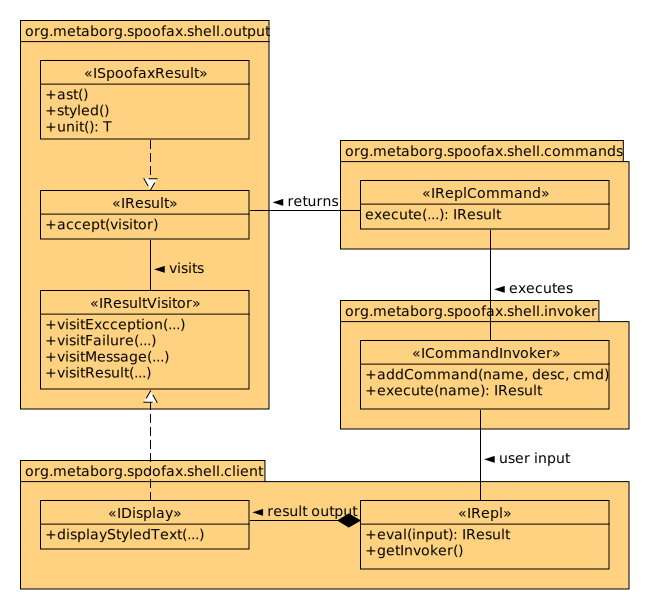
\includegraphics[width=0.75\textwidth]{uml-overview}
  \caption{An overview of the most relevant components of the product.}
  \label{fig:uml-overview}
\end{figure}
